 \documentclass[12pt]{article}
 \usepackage{pstricks,pst-node,pst-tree}
 \usepackage{geometry}
\usepackage{graphicx}
 \usepackage{lscape}
\usepackage{appendix}
\title{Mississippi}
\definecolor{wheat}{rgb}{0.96, 0.87, 0.7}
\pagestyle{empty}
\begin{document}
\maketitle{}
\newpage
\tableofcontents
\newpage
\section{Summary}
This article is trying to show estimate $\mu$ (state population mean)of INTP(interest, dividends,and net rental income past 12months)with sampling weight $\omega_i$ in variable PWGTP by using the PERSON RECORD variables of Mississippi. The method is that use GUIDE to estimate π (probability of response), then use the inverse probability weighted (IPW) method to estimate $\mu$. First, we need to do the data cleaning since there are 286 variables and over 27000 observations. Then we need to assign each variable with a proper index, which shows the type that the variable belongs to. After that, we can use GUIDE to output the classification tree. In addition, we use GUIDE to produce regression as well as linear and logistic regression in R in order to make comparison and discuss the result. 
\section{Data Cleaning}
In order to use GUIDE to run classsificaion tree,we need to create a description file in advanced. The catogories are listed in the appendix\\
When we are constructing classification tree, we use INTP \_ as dependent variable, while doing regression, we use INTP.
\section{Classification Tree}
 \begin{center}
\psset{linecolor=black,tnsep=1pt,tndepth=0cm,tnheight=0cm,treesep=.8cm,levelsep=56pt,radius=10pt}
  \pstree[treemode=D]{\Tcircle{ 1 }~[tnpos=l]{\shortstack[r]{\texttt{\detokenize{PAP}}= \texttt{\detokenize{NA}}}}
    ~[tnpos=r]{\shortstack[r]{0.16\\0.84}}}{
  \pstree[treemode=D]{\Tcircle{ 2 }~[tnpos=l]{\shortstack[r]{\texttt{\detokenize{SSP}}= \texttt{\detokenize{NA}}}}
 }{
 \Tcircle[fillcolor=yellow,fillstyle=solid]{ 4 }
    ~[tnpos=l]{\shortstack[r]{0.97\\0.03}}
    ~{\shortstack{\makebox[0pt][c]{\texttt{\detokenize{0}}}2978}}
  \pstree[treemode=D]{\Tcircle{ 5 }~[tnpos=l]{\shortstack[r]{\texttt{\detokenize{RETP}}$\leq$1050}}
 }{
 \Tcircle[fillcolor=green,fillstyle=solid]{\small 10}
    ~[tnpos=l]{\shortstack[r]{0.17\\0.83}}
    ~{\shortstack{\makebox[0pt][c]{\texttt{\detokenize{1}}}121}}
 \Tcircle[fillcolor=yellow,fillstyle=solid]{\small 11}
    ~[tnpos=r]{\shortstack[r]{0.58\\0.42}}
    ~{\shortstack{\makebox[0pt][c]{\texttt{\detokenize{0}}}231}}
   }
   }
  \pstree[treemode=D]{\Tcircle{ 3 }~[tnpos=l]{\shortstack[r]{\texttt{\detokenize{PINCP}}= \texttt{\detokenize{NA}}}}
 }{
  \pstree[treemode=D]{\Tcircle{ 6 }~[tnpos=l]{\shortstack[r]{\texttt{\detokenize{PERNP}}= \texttt{\detokenize{NA}}}}
 }{
 \Tcircle[fillcolor=green,fillstyle=solid]{\small 12}
    ~[tnpos=l]{\shortstack[r]{0.08\\0.92}}
    ~{\shortstack{\makebox[0pt][c]{\texttt{\detokenize{1}}}2293}}
  \pstree[treemode=D]{\Tcircle{\small 13}~[tnpos=l]{\shortstack[r]{\texttt{\detokenize{SSP}}= \texttt{\detokenize{NA}}}}
 }{
 \Tcircle[fillcolor=green,fillstyle=solid]{\small 26}
    ~[tnpos=l]{\shortstack[r]{0.15\\0.85}}
    ~{\shortstack{\makebox[0pt][c]{\texttt{\detokenize{1}}}803}}
  \pstree[treemode=D]{\Tcircle{\small 27}~[tnpos=l]{\shortstack[r]{\texttt{\detokenize{RETP}}= \texttt{\detokenize{NA}}}}
 }{
 \Tcircle[fillcolor=green,fillstyle=solid]{\small 54}
    ~[tnpos=l]{\shortstack[r]{0.11\\0.89}}
    ~{\shortstack{\makebox[0pt][c]{\texttt{\detokenize{1}}}199}}
  \pstree[treemode=D]{\Tcircle{\small 55}~[tnpos=l]{\shortstack[r]{\texttt{\detokenize{SSIP}}= \texttt{\detokenize{NA}}}}
 }{
 \Tcircle[fillcolor=green,fillstyle=solid]{\tiny 110}
    ~[tnpos=l]{\shortstack[r]{0.12\\0.88}}
    ~{\shortstack{\makebox[0pt][c]{\texttt{\detokenize{1}}}137}}
 \Tcircle[fillcolor=yellow,fillstyle=solid]{\tiny 111}
    ~[tnpos=r]{\shortstack[r]{0.84\\0.16}}
    ~{\shortstack{\makebox[0pt][c]{\texttt{\detokenize{0}}}489}}
   }
   }
   }
   }
 \Tcircle[fillcolor=green,fillstyle=solid]{ 7 }
    ~[tnpos=r]{\shortstack[r]{0.00\\1.00}}
    ~{\shortstack{\makebox[0pt][c]{\texttt{\detokenize{1}}}16787}}
 }
 }
 \end{center}
GUIDE v.32.0  0.50-SE
classification tree for predicting \texttt{\detokenize{INTP \_ }} using
estimated priors
and unit misclassification costs.
 Number of observations used to contruct tree is 24038.
 Maximum number of split levels is 30 and minimum node sample size is 120.
At each split, an observation goes to the left branch 
 if and only if the condition is satisfied.
Predicted classes and sample sizes printed below terminal nodes;
 class proportions for \texttt{\detokenize{INTP \_ }} =
 \texttt{\detokenize{0}} and \texttt{\detokenize{1}} beside nodes.
Second best split variable at root node is \texttt{\detokenize{OIP}}.
\section{GUIDE Regression}
 \begin{center}
\psset{linecolor=black,tnsep=1pt,tndepth=0cm,tnheight=0cm,treesep=.8cm,levelsep=50pt,radius=10pt}
  \pstree[treemode=D]{\TC~[tnpos=l]{\shortstack[r]{\texttt{\detokenize{PINCP}}$\leq_*$289500}}
 }{
    \TC[fillcolor=yellow,fillstyle=solid]~{\shortstack[c]{\emph{20057}459.5}}
    \TC[fillcolor=yellow,fillstyle=solid]~{\shortstack[c]{\emph{181}71208.}}
 }
 \end{center}
GUIDE v.32.0  0.20-SE
piecewise constant least-squares regression tree
for predicting \texttt{\detokenize{INTP}}.
 Number of observations used to contruct tree is 20238
 (excluding observations with non-positive weight or with missing values
 in d, t, r or z variables).
 Maximum number of split levels is 30 and minimum node sample size is 101.
At each split, an observation goes to the left branch 
 if and only if the condition is satisfied.
 The symbol `$\leq_*$' stands for `$\leq$ or missing'.
Sample size (\emph{in italics}) and mean of \texttt{\detokenize{INTP}} printed below nodes.
Second best split variable at root node is \texttt{\detokenize{POVPIP}}.
\section{Logistic Regression in R}
In the following two sections, logistic and linear regression will be shown. However before that, I run important score in GUIDE to determine how many variable are "important", so that we can simplified the model. The graph of important scores are shown below:
\newline
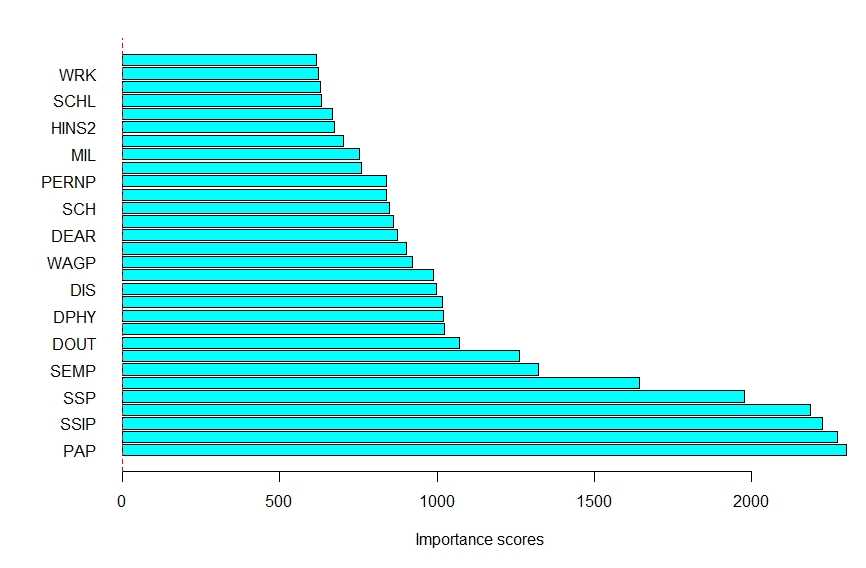
\includegraphics[height=8cm,width=12cm]{imp.jpeg}
\newline
Belows are the summary of Logistic Regression:\\
Call:\\
glm(formula = INTP \_  ~ ., family = binomial(link = "logit"), data = datLogistic)\\
Deviance Residuals: \\
    Min       1Q   Median       3Q      Max  \\
-3.5933   0.2853   0.3917   0.5251   2.4313  \\
Coefficients: (3 not defined because of singularities)\\
              Estimate Std. Error z value Pr(>|z|)\\
(Intercept) -2.314e+01  1.549e+00 -14.939  < 2e-16\\
DRAT1       -6.675e-02  5.263e-01  -0.127  0.89907\\
DRAT2        9.537e-01  3.853e-01   2.475  0.01332\\
DRAT3        5.950e-01  4.447e-01   1.338  0.18095\\
DRAT4        1.338e+00  5.978e-01   2.238  0.02521\\
DRAT5        1.869e-01  2.779e-01   0.673  0.50110\\
DRAT6       -7.219e-02  5.866e-01  -0.123  0.90205\\
HINS21       1.162e+00  9.110e-02  12.751  < 2e-16\\
HINS22       1.399e+00  9.792e-02  14.291  < 2e-16\\
HINS41       1.123e+00  1.038e-01  10.823  < 2e-16\\
HINS42       5.736e-01  1.106e-01   5.188 2.13e-07\\
HINS51       8.990e-01  1.560e-01   5.764 8.21e-09\\
HINS52       5.307e-01  1.782e-01   2.978  0.00290\\
HINS61       7.350e-01  1.748e-01   4.204 2.62e-05\\
HINS62       5.377e-01  1.990e-01   2.702  0.00689\\
HINS71       9.433e-02  4.094e-01   0.230  0.81779\\
HINS72      -1.530e-01  2.190e-01  -0.699  0.48472\\
MARHYP       1.143e-02  7.926e-04  14.422  < 2e-16\\
MLPE0        6.128e-01  1.293e+00   0.474  0.63549\\
MLPE1       -1.759e+00  1.699e+00  -1.035  0.30060\\
MLPFG0       4.642e-01  3.550e-01   1.308  0.19097\\
MLPFG1              NA         NA      NA       NA\\
RETP         3.068e-05  4.250e-06   7.217 5.30e-13\\
SSP          1.073e-04  5.327e-06  20.138  < 2e-16\\
DECADE1      7.993e-01  1.147e+00   0.697  0.48581\\
DECADE2     -5.076e-01  5.173e-01  -0.981  0.32648\\
DECADE3     -1.112e-01  3.946e-01  -0.282  0.77815\\
DECADE4      8.664e-02  4.350e-01   0.199  0.84215\\
DECADE5     -1.824e-01  3.116e-01  -0.585  0.55843\\
DECADE6      3.839e-01  3.179e-01   1.208  0.22712\\
DECADE7      3.531e-01  3.063e-01   1.153  0.24898\\
DECADE8      4.979e-01  2.546e-01   1.955  0.05054\\
SCIENGRLP1  -1.722e-02  1.401e-01  -0.123  0.90218\\
SCIENGRLP2   1.502e-02  5.816e-02   0.258  0.79618\\
VPS1        -1.260e+00  1.263e+00  -0.997  0.31862\\
VPS2        -1.951e+00  1.270e+00  -1.537  0.12441\\
VPS3         1.784e+00  1.925e+00   0.927  0.35403\\
VPS4        -8.396e-01  1.270e+00  -0.661  0.50839\\
VPS5         3.624e-01  1.786e+00   0.203  0.83922\\
VPS6         1.073e+00  1.732e+00   0.620  0.53532\\
VPS7         9.051e-01  1.787e+00   0.507  0.61250\\
VPS8                NA         NA      NA       NA\\
VPS9        -1.523e+00  1.270e+00  -1.200  0.23032\\
VPS10       -3.319e+00  1.590e+00  -2.087  0.03691\\
VPS11       -1.407e+00  1.309e+00  -1.075  0.28243\\
VPS12       -9.343e-01  1.262e+00  -0.740  0.45913\\
VPS13       -5.187e-01  1.316e+00  -0.394  0.69337\\
VPS14               NA         NA      NA       NA\\
FHINS3C0    -7.390e-01  5.784e-02 -12.775  < 2e-16\\
FHINS3C1    -1.925e+00  1.558e-01 -12.358  < 2e-16\\
               \\
(Intercept) ***\\
DRAT1          \\
DRAT2       *  \\
DRAT3          \\
DRAT4       *  \\
DRAT5          \\
DRAT6          \\
HINS21      ***\\
HINS22      ***\\
HINS41      ***\\
HINS42      ***\\
HINS51      ***\\
HINS52      ** \\
HINS61      ***\\
HINS62      ** \\
HINS71         \\
HINS72         \\
MARHYP      ***\\
MLPE0          \\
MLPE1          \\
MLPFG0         \\
MLPFG1         \\
RETP        ***\\
SSP         ***\\
DECADE1        \\
DECADE2        \\
DECADE3        \\
DECADE4        \\
DECADE5        \\
DECADE6        \\
DECADE7        \\
DECADE8     .  \\
SCIENGRLP1     \\
SCIENGRLP2     \\
VPS1           \\
VPS2           \\
VPS3           \\
VPS4           \\
VPS5           \\
VPS6           \\
VPS7           \\
VPS8           \\
VPS9           \\
VPS10       *  \\
VPS11          \\
VPS12          \\
VPS13          \\
VPS14          \\
FHINS3C0    ***\\
FHINS3C1    ***\\
---
Signif. codes:  \\
0 ‘***’ 0.001 ‘**’ 0.01 ‘*’ 0.05 ‘.’ 0.1 ‘ ’ 1\\

(Dispersion parameter for binomial family taken to be 1)\\

    Null deviance: 20984  on 24037  degrees of freedom\\
Residual deviance: 15940  on 23991  degrees of freedom\\
AIC: 16034\\

Number of Fisher Scoring iterations: 6\\

 20238\\
1000.062\\
0.8870538\\
\section{Linear Regression in R}
> summary(predict(a))\\
     Min.   1st Qu.    Median      Mean   3rd Qu.      Max. \\
-150882.4    -719.2     612.7     786.2    2468.0  171087.3\\ 
\section{Comparison}
In GUIDE classification: the mean of INTP is\\ 
\begin{center}
> uclass\\
1086.261\\
\end{center}
In GUIDE regression: the mean of INTP is\\
\begin{center}
> uregression\\
921.2957\\
\end{center}
In R logistic regression: the mean of INTP is\\
\begin{center}
>rlogistic\\
1000.062\\
\end{center}
In R linear regression: the mean of INTP is\\
\begin{center}
>rlinear\\
786.2\\
\end{center}
According to the code:\\
\begin{center}
mu.gov = sum(rawdataG\$PWGTP*rawdataG\$INTP)/sum(rawdataG\$PWGTP)
\end{center}
we have the mean of INTP\\
> mu.gov\\
1099.817\\
\section{Conclusion}
Comparing to mu.gov, we can see the classification has the closest estimation. And the regression in GUIDE has the second close to mu.gov. However, the linear regression does not fit the model well this may be caused by two factors. One is that we only use some "important" variables rather than entire explanatory variables, this leads to some imformation lost. Another reason is that there are too many missing values and we have add some values not from the real record. Thus, the data can be non-linearity and the linear regression does not fit.
\newpage
\appendixpage
\section{Data Cleaning}
RT x\\
SERIALNO x\\ 
DIVISION x\\
SPORDER x\\
PUMA x\\
REGION x\\
ST x\\
ADJINC x\\
PWGTP w\\
1AGEP n\\
CIT b\\
 CITWP n\\
COW b\\
DDRS b\\
DEAR b\\
DEYE b\\
DOUT b\\
DPHY b\\
DRAT b\\
DRATX b\\
DREM b\\
ENG b\\
FER b\\
GCL b\\
GCM b\\
GCR b\\
HINS1 b\\
HINS2 b\\
HINS3 b\\
HINS4 b\\
HINS5 b\\
HINS6 b\\
HINS7 b\\
INTP x\\
JWMNP n\\
JWRIP n\\
JWTR b\\
LANX b\\
MAR b\\
MARHD b\\
MARHM b\\
MARHT b\\
MARHW b\\
MARHYP n\\
MIG b\\
MIL b\\
MLPA b\\
MLPB b\\
MLPCD b\\
MLPE b\\
MLPFG b\\
MLPH b\\
MLPI b\\
MLPJ b\\
MLPK b\\
NWAB b\\
NWAV b\\
NWLA b\\
NWLK b\\
NWRE b\\
OIP n\\
PAP n\\
RELP b\\
RETP n\\
SCH b\\
SCHG b\\
SCHL b\\
SEMP n\\
SEX b\\
SSIP n\\
SSP n\\
WAGP n\\
WKHP n\\
WKL b\\
WKW b\\
WRK b\\
YOEP n\\
ANC b\\
ANC1P b\\
ANC2P b\\
DECADE b\\
DIS b\\
DRIVESP b\\
ESP b\\
ESR b\\
FOD1P b\\
FOD2P b\\
HICOV b\\
HISP b\\
INDP b\\
JWAP p 286\\
JWDP p 151\\
LANP b\\
MIGPUMA b\\
MIGSP b\\
MSP b\\
NATIVITY b\\
NOP b\\
OC b\\
OCCP b\\
PAOC b\\
PERNP n\\
PINCP n\\
POBP b\\
POVPIP n\\
POWPUMA b\\
POWSP b\\
PRIVCOV b\\
PUBCOV b\\
QTRBIR b\\
RAC1P b\\
RAC2P b\\
RAC3P b\\
RACAIAN b\\
RACASN b\\
RACBLK b\\
RACNH b\\
RACNUM b\\
RACPI b\\
RACSOR b\\
RACWHT b\\
RC b\\
SCIENGP b\\
SCIENGRLP b\\
SFN b\\
SFR b\\
VPS b\\
WAOB b\\
FAGEP x\\
FANCP x\\
FCITP x\\
FCITWP x\\
FCOWP x\\
FDDRSP x\\
FDEARP x\\
FDEYEP x\\
FDISP x\\
FDOUTP x\\
FDPHYP x\\
FDRATP x\\
FDRATXP x\\
FDREMP x\\
FENGP x\\
FESRP x\\
FFERP x\\
FFODP b\\
FGCLP x\\
FGCMP x\\
FGCRP x\\
FHICOVP x\\
FHINS1P x\\
FHINS2P x\\
FHINS3C b\\
FHINS3P x\\
FHINS4C b\\
FHINS4P x\\
FHINS5C b\\
FHINS5P x\\
FHINS6P x\\
FHINS7P x\\
FHISP x\\
FINDP x\\
INTP x\\
FJWDP x\\
FJWMNP x\\
FJWRIP x\\
FJWTRP x\\
FLANP x\\
FLANXP x\\
FMARP x\\
FMARHDP x\\
FMARHMP x\\
FMARHTP x\\
FMARHWP x\\
FMARHYP x\\
FMIGP x\\
FMIGSP x\\
FMILPP b\\
FMILSP x\\
FOCCP x\\
FOIP x\\
FPAP x\\
FPERNP x\\
FPINCP x\\
FPOBP x\\
FPOWSP x\\
FPRIVCOVP x\\
FPUBCOVP x\\
FRACP x\\
FRELP x\\
FRETP x\\
FSCHGP x\\
FSCHLP x\\
FSCHP x\\
FSEMP x\\
FSEXP x\\
FSSIP x\\
FSSP x\\
FWAGP x\\
FWKHP x\\
FWKLP x\\
FWKWP x\\
FWRKP x\\
FYOEP x\\
PWGTP1 x\\
PWGTP2 x\\
PWGTP3 x\\
PWGTP4 x\\
PWGTP5 x\\
PWGTP6 x\\
PWGTP7 x\\
PWGTP8 x\\
PWGTP9 x\\
PWGTP10 x\\
PWGTP11 x\\
PWGTP12 x\\
PWGTP13 x\\
PWGTP14 x\\
PWGTP15 x\\
PWGTP16 x\\
PWGTP17 x\\
PWGTP18 x\\
PWGTP19 x\\
PWGTP20 x\\
PWGTP21 x\\
PWGTP22 x\\
PWGTP23 x\\
PWGTP24 x\\
PWGTP25 x\\
PWGTP26 x\\
PWGTP27 x\\
PWGTP28 x\\
PWGTP29 x\\
PWGTP30 x\\
PWGTP31 x\\
PWGTP32 x\\
PWGTP33 x\\
PWGTP34 x\\
PWGTP35 x\\
PWGTP36 x\\
PWGTP37 x\\
PWGTP38 x\\
PWGTP39 x\\
PWGTP40 x\\
PWGTP41 x\\
PWGTP42 x\\
PWGTP43 x\\
PWGTP44 x\\
PWGTP45 x\\
PWGTP46 x\\
PWGTP47 x\\
PWGTP48 x\\
PWGTP49 x\\
PWGTP50 x\\
PWGTP51 x\\
PWGTP52 x\\
PWGTP53 x\\
PWGTP54 x\\
PWGTP55 x\\
PWGTP56 x\\
PWGTP57 x\\
PWGTP58 x\\
PWGTP59 x\\
PWGTP60 x\\
PWGTP61 x\\
PWGTP62 x\\
PWGTP63 x\\
PWGTP64 x\\
PWGTP65 x\\
PWGTP66 x\\
PWGTP67 x\\
PWGTP68 x\\
PWGTP69 x\\
PWGTP70 x\\
PWGTP71 x\\
PWGTP72 x\\
PWGTP73 x\\
PWGTP74 x\\
PWGTP75 x\\
PWGTP76 x\\
PWGTP77 x\\
PWGTP78 x\\
PWGTP79 x\\
PWGTP80 x\\
INTP \_  d\\
\section{All R codes}
rawdata = read.csv("psam\_p28.csv", head = TRUE)\\
rawdataG = rawdata[-which(rawdata\$AGEP<15),]\\
mu.gov = sum(rawdataG\$PWGTP*rawdataG\$INTP)/sum(rawdataG\$PWGTP)\\
rawdataAl = rawdata\\
rawdataAl = rawdataAl[-which(rawdataAl\$AGEP<15),]
\\Flagname = c()
\\for (i in (grep("FAGEP",colnames(rawdataAl)):grep("FYOEP",colnames(rawdataAl)))) {
  \\Flagname[i+1-grep("FAGEP",colnames(rawdataAl))] = unlist(strsplit(colnames(rawdataAl[i]),split = "F",fixed = T))[2]
}
Flagname[17] = "FERP"\\
Flagname[18] = "FODP"\\
Flagname1 = data.frame(Rawname = rep(NA,length(Flagname)),Flagname = rep(NA,length(Flagname)),Rawnum = rep(0,length(Flagname)),Flagnum = c(grep("FAGEP",colnames(rawdataAl)):grep("FYOEP",colnames(rawdataAl))))
\\for (i in 1:length(Flagname)) {
  \\a = grep(Flagname[i],colnames(rawdataAl),value = T,fixed=T)
  \\b = grep(Flagname[i],colnames(rawdataAl),fixed=T)
  \\if(length(a) == 2){
    \\Flagname1\$Rawname[i] = a[1]
    \\Flagname1\$Flagname[i] = a[2]
    Flagname1\$Rawnum[i] = b[1]\\
  }else if(length(a) == 1){\\
    Flagname1\$Rawname[i] = NA\\
    Flagname1\$Flagname[i] = a[1]\\
    print(isTRUE(b[1]==Flagname1\$Flagnum[i]))
  \\}else{print(a)}
}
Flagname1[which(Flagname1\$Flagname=="FANCP"),1]="ANC"\\
Flagname1[which(Flagname1\$Flagname=="FCITP"),1]="CIT"\\
Flagname1[which(Flagname1\$Flagname=="FCOWP"),1]="COW"\\
Flagname1[which(Flagname1\$Flagname=="FDDRSP"),1]="DDRS"\\
Flagname1[which(Flagname1\$Flagname=="FDEARP"),1]="DEAR"\\
Flagname1[which(Flagname1\$Flagname=="FDEYEP"),1]="DEYE"\\
Flagname1[which(Flagname1\$Flagname=="FDISP"),1]="DIS"\\
Flagname1[which(Flagname1\$Flagname=="FDOUTP"),1]="DOUT"\\
Flagname1[which(Flagname1\$Flagname=="FDPHYP"),1]="DPHY"\\
Flagname1[which(Flagname1\$Flagname=="FDRATP"),1]="DRAT"\\
Flagname1[which(Flagname1\$Flagname=="FDRATXP"),1]="DRATX"\\
Flagname1[which(Flagname1\$Flagname=="FDREMP"),1]="DREM"\\
Flagname1[which(Flagname1\$Flagname=="FESRP"),1]="ESR"\\
Flagname1[which(Flagname1\$Flagname=="FFERP"),1]="FER"\\
Flagname1[which(Flagname1\$Flagname=="FGCLP"),1]="GCL"\\
Flagname1[which(Flagname1\$Flagname=="FGCMP"),1]="GCM"\\
Flagname1[which(Flagname1\$Flagname=="FGCRP"),1]="GCR"\\
Flagname1[which(Flagname1\$Flagname=="FHICOVP"),1]="HICOV"\\
Flagname1[which(Flagname1\$Flagname=="FHINS1P"),1]="HINS1"\\
Flagname1[which(Flagname1\$Flagname=="FHINS2P"),1]="HINS2"\\
Flagname1[which(Flagname1\$Flagname=="FHINS3P"),1]="HINS3"\\
Flagname1[which(Flagname1\$Flagname=="FHINS4P"),1]="HINS4"\\
Flagname1[which(Flagname1\$Flagname=="FHINS5P"),1]="HINS5"\\
Flagname1[which(Flagname1\$Flagname=="FHINS6P"),1]="HINS6"\\
Flagname1[which(Flagname1\$Flagname=="FHINS7P"),1]="HINS7"\\
Flagname1[which(Flagname1\$Flagname=="FJWTRP"),1]="JWTR"\\
Flagname1[which(Flagname1\$Flagname=="FLANXP"),1]="LANX"\\
Flagname1[which(Flagname1\$Flagname=="FMARP"),1]="MAR"\\
Flagname1[which(Flagname1\$Flagname=="FMARHDP"),1]="MARHD"\\
Flagname1[which(Flagname1\$Flagname=="FMARHMP"),1]="MARHM"\\
Flagname1[which(Flagname1\$Flagname=="FMARHTP"),1]="MARHT"\\
Flagname1[which(Flagname1\$Flagname=="FMARHWP"),1]="MARHW"\\
Flagname1[which(Flagname1\$Flagname=="FMILSP"),1]="MIL"\\
Flagname1[which(Flagname1\$Flagname=="FPRIVCOVP"),1]="PRIVCOV"\\
Flagname1[which(Flagname1\$Flagname=="FPUBCOVP"),1]="PUBCOV"\\
Flagname1[which(Flagname1\$Flagname=="FSCHGP"),1]="SCHG"\\
Flagname1[which(Flagname1\$Flagname=="FSCHLP"),1]="SCHL"\\
Flagname1[which(Flagname1\$Flagname=="FSCHP"),1]="SCH"\\
Flagname1[which(Flagname1\$Flagname=="FSEXP"),1]="SEX"\\
Flagname1[which(Flagname1\$Flagname=="FWKLP"),1]="WKL"\\
Flagname1[which(Flagname1\$Flagname=="FWKWP"),1]="WKW"\\
Flagname1[which(Flagname1\$Flagname=="FWRKP"),1]="WRK"\\
for (i in 1:nrow(Flagname1)) {\\
  if(i \%in\% c(18,25,27,29,50)){next}
  if(Flagname1\$Rawname[i]\%in\% colnames(rawdataAl)){Flagname1\$Rawnum[i]= which(colnames(rawdataAl)==Flagname1\$Rawname[i])}
}
for (i in 1:nrow(Flagname1)){\\
  if(i \%in\% c(18,25,27,29,50)){next}
\\  for (j in 1:nrow(rawdataAl)) {
  \\  if(rawdataAl[j,Flagname1\$Flagnum[i]]==1){
    \\  rawdataAl[j,Flagname1\$Rawnum[i]] = NA
    \\}
  }
}
dat = rawdataAl\\
dat\$INTP \_  = ifelse(is.na(dat\$INTP), 0, 1)\\
dat0 = dat\\
dat = dat[,-c(97,128)]\\
write.table(dat, file = "model.txt",row.names=F)\\
k = ncol(dat)\\
roles = rep("n",k)\\
b.vars =\\ c("CIT","COW","DDRS","DEAR","DEYE","DOUT","DPHY","DRAT","DRATX","DREM","ENG","FER","GCL","GCM","GCR","HINS1","HINS2","HINS3","HINS4","HINS5","HINS6","HINS7",
           "JWTR","LANX","MAR","MARHD","MARHM","MARHT","MARHW","MIG","MIL","MLPA","MLPB","MLPCD","MLPE","MLPFG","MLPH","MLPI","MLPJ","MLPK","NWAB","NWAV","NWLA","NWLK",
           "NWRE","RELP","SCH","SCHG","SCHL","SEX","WKL","WKW","WRK","ANC","ANC1P","ANC2P","DECADE","DIS","DRIVESP","ESP","ESR","FOD1P","FOD2P","HICOV","HISP","INDP",
           "LANP","MIGPUMA","MIGSP","MSP","NATIVITY","NOP","OC","OCCP","PAOC","POBP","POWPUMA","POWSP","PRIVCOV","PUBCOV","QTRBIR","RAC1P","RAC2P","RAC3P",
           "RACAIAN","RACASN","RACBLK","RACNH","RACNUM","RACPI","RACSOR","RACWHT","RC","SCIENGP","SCIENGRLP","SFN","SFR","VPS","WAOB","FFODP","FHINS3C","FHINS4C","FHINS5C",
           "FMILPP") \\
roles[names(dat) \%in\% b.vars] = "b"\\
n.vars = c("AGEP","CITWP","JWMNP","JWRIP","MARHYP","OIP","PAP","RETP","SEMP","SSIP","SSP","WAGP","WKHP","YOEP","PERNP","PINCP","POVPIP") \\
roles[names(dat) \%in\% n.vars] = "n"\\
p.vars1 = "JWAP"\\
p.vars2 = "JWDP"\\
roles[names(dat) \%in\% p.vars1] = "p 286\\
roles[names(dat) \%in\% p.vars2] = "p 151"\\
i = c(1:80)\\
PWGTPX = paste("PWGTP",i,sep = "")\\
x.vars = c("SPORDER","PUMA","RT","SERIALNO","DIVISION","REGION","ST","ADJINC","INTP",Flagname1[-c(18,25,27,29,50),][,2],PWGTPX) \\
roles[names(dat) \%in\% x.vars] = "x"\\
d.var = "INTP \_ "\\
roles[names(dat) \%in\% d.var] = "d"\\
w.var = "PWGTP"\\
roles[names(dat) \%in\% w.var] = "w"\\
write("model.txt",file="desc.txt") \\
write("NA",file="desc.txt",append=TRUE) \\
write("2",file="desc.txt",append=TRUE) \\
write.table(cbind(1:k,names(dat),roles),file="desc.txt",\\
            row.names=FALSE,col.names=FALSE,quote=FALSE,append=TRUE)\\
exclude1 = c("SPORDER","PUMA","RT","SERIALNO","DIVISION","REGION","ST","ADJINC")\\
i = c(1:80)\\
exclude2 = paste("PWGTP",i,sep = "")\\
exclude3 = c("INDP","MIGPUMA","MIGSP","OCCP","POBP")\\
exclude = c(exclude1,exclude2,exclude3)\\
datR = dat[,-which(names(dat) \%in\% exclude)]\\
for (i in 1:ncol(datR)) {\\
  index = which(is.na(datR[,i]))\\
  datR[index,i]=min(datR[,i],na.rm = T)-1\\
}
a=lm(datR\$INTP~datR\$FOD1P+datR\$FOD2P+datR\$ANC1P+datR\$ANC2P+datR\$VPS+datR\$LANP+datR\$DRAT+datR\$DECADE+datR\$HINS2+datR\$FHINS3C+datR\$HINS5+datR\$HINS6+datR\$HINS7+datR\$MLPFG+datR\$MARHYP+datR\$HINS4+datR\$MLPE+datR\$SCIENGP+datR\$RETP+datR\$SSP+datR\$MLPH+datR\$MLPJ+datR\$SCIENGP+datR\$PINCP+datR\$DRATX+datR\$PRIVCOV+datR\$PUBCOV+datR\$MLPCD+datR\$MARHW+datR\$OIP+datR\$POVPIP+datR\$SEMP+datR\$MLPI+datR\$HINS3+datR\$AGEP+datR\$HICOV+datR\$MLPK+datR\$HINS1+datR\$MLPA+datR\$MLPB+datR\$RACBLK+datR\$RACWHT+datR\$COW+datR\$MIL+datR\$NWAV+datR\$MARHT+datR\$MSP+datR\$CITWP+datR\$MAR+datR\$ANC+datR\$FFODP+datR\$MARHM+datR\$RACASN+datR\$WKL+datR\$DIS+datR\$PERNP+datR\$WKHP+datR\$FMILPP+datR\$RACNH+datR\$QTRBIR+datR\$WAGP+datR\$JWAP+datR\$JWDP+datR\$JWTR+datR\$ESP+datR\$ESR+datR\$SFR+datR\$RACNUM+datR\$GCM+datR\$DRIVESP+datR\$CIT+datR\$RELP+datR\$SEX+datR\$RAC1P+datR\$RACPI+datR\$ENG+datR\$MIG+datR\$SFN+datR\$FHINS5C+datR\$RACAIAN+datR\$NWRE+datR\$RACSOR+datR\$DEAR+datR\$OC+datR\$SCH+datR\$GCR+datR\$DEYE+datR\$DOUT+datR\$LANX+datR\$NWAB+datR\$DREM+datR\$DDRS+datR\$NWLA+datR\$DPHY+datR\$PAP+datR\$SSIP+datR\$YOEP+datR\$RC+datR\$NWLK+datR\$MARHD+datR\$FER+datR\$WKW+datR\$JWRIP+datR\$NATIVITY+datR\$PAOC+datR\$FHINS4C+datR\$GCL+datR\$WRK+datR\$JWMNP)\\
summary(a)\\
z0 <- read.table("imp.scr",header=TRUE) \\
par(mar=c(5,6,2,1),las=1) \\
barplot(z0\$Score[1:30],names.arg=z0\$Variable[1:30],col="cyan",horiz=TRUE,xlab="Importance scores") \\
abline(v=1,col="red",lty=2)\\
v.score = as.character(z0\$Variable[1:100])\\
v = c(v.score,"INTP \_ ")\\
datLogistic = datR[,which(names(datR) \%in\% v)]\\
for(i in which(names(datLogistic) \%in\% v)){\\
  datLogistic[,i] = as.factor(datLogistic[,i])\\
}
model = glm(INTP \_  ~.,\\
            data=datLogistic,\\
            family = binomial(link = "logit")\\
)\\
summary(model)\\
pifile=read.table("MS.FIT",header = T)\
regressionfile=read.table("regression.fit",header = T)\\
regression=regressionfile\$predicted[regressionfile\$train=="n"]\\
na=0\\
nonna=0\\
pwgtpna=dat\$PWGTP[is.na(dat\$INTP)]\\
pwgtpnonna=dat\$PWGTP[is.na(dat\$INTP)==F]\\
intpnonna=dat\$INTP[is.na(dat\$INTP)==F]\\
for (i in 1:3800) {\\
  na=na+regression[i]*pwgtpna[i]\\
}
for (i in 1:20238) {\\
  nonna=nonna+intpnonna[i]*pwgtpnonna[i]\\
}
uregression=(na+nonna)/sum(dat\$PWGTP)\\
pi=pifile\$X1/(pifile\$X1+pifile\$X0)\\
divide=0\\
multi=0\\
for (i in which(is.na(dat\$INTP)==F)) {\\
  divide=divide+datR\$PWGTP[i]/pi[i]\\
  multi=multi+(datR\$PWGTP[i]*datR\$INTP[i])/pi[i]\\
}
uclass=multi/divide\\
\section{Classification Input and Output Files}
\subsection{Input}
GUIDE       (do not edit this file unless you know what you are doing)\\
  32.0      (version of GUIDE that generated this file)\\
 1          (1=model fitting, 2=importance or DIF scoring, 3=data conversion)\\
"MS.out"  (name of output file)\\
 1          (1=one tree, 2=ensemble)\\
 1          (1=classification, 2=regression, 3=propensity score grouping)\\
 1          (1=simple model, 2=nearest-neighbor, 3=kernel)\\
 1          (0=linear 1st, 1=univariate 1st, 2=skip linear, 3=skip linear and interaction)\\
 1          (1=prune by CV, 2=by test sample, 3=no pruning)\\
"desc.txt"  (name of data description file)\\
        10  (number of cross-validations)\\
 1          (1=mean-based CV tree, 2=median-based CV tree)\\
     0.500  (SE number for pruning)\\
 1          (1=estimated priors, 2=equal priors, 3=other priors)\\
 1          (1=unit misclassification costs, 2=other)\\
 2          (1=split point from quantiles, 2=use exhaustive search)\\
 1          (1=default max. number of split levels, 2=specify no. in next line)\\
 1          (1=default min. node size, 2=specify min. value in next line)\\
 1          (1=write latex, 2=skip latex)\\
"MS.tex" (latex file name)\\
 1          (1=include node numbers, 2=exclude)\\
 1          (1=number all nodes, 2=only terminal nodes)\\
 1          (1=color terminal nodes, 2=no colors)\\
 1          (0=\# errors, 1=class sizes in nodes, 2=nothing)\\
 1          (1=no storage, 2=store fit and split variables, 3=store split variables and values)\\
 2          (1=do not save fitted values and node IDs, 2=save in a file)\\
"MS.FIT" (file name for fitted values and node IDs)\\
 2          (1=do not write R function, 2=write R function)\\
"MS.r" (R code file)\\
 1          (rank of top variable to split root node)\\
\subsection{Output}
             GGG   U   U  I  DDDD   EEEE\\
            G   G  U   U  I  D   D  E\\
            G      U   U  I  D   D  E\\
            G  GG  U   U  I  D   D  EEE\\
            G   G  U   U  I  D   D  E\\
            G   G  U   U  I  D   D  E\\
             GGG    UUU   I  DDDD   EEEE
   
 GUIDE Classification and Regression Trees and Forests\\
 Version 32.0 (Build date: August 29, 2019)        \\
 Compiled with Visual Fortran 64 18.0.1.156 on Windows 10\\              
 Copyright (c) 1997-2019 Wei-Yin Loh. All rights reserved.\\
 This software is based upon work supported by the U.S. Army Research Office,\\
 the National Science Foundation and the National Institutes of Health.\\
  
 This job was started on 10/31/19 at 17:37
  
 Classification tree\\
 Pruning by cross-validation\\
 Data description file: desc.txt\\
 Training sample file: model.txt\\
 Missing value code: NA\\
 Records in data file start on line 2\\
 Warning: N variables changed to S\\
 Warning: B variables changed to C\\
 Dependent variable is INTP \_ \\
 Number of records in data file: 24038\\
 Length of longest entry in data file: 13\\
 Missing values found among categorical variables\\
 Separate categories will be created for missing categorical variables\\
 Number of classes: 2\\
 Smallest and largest positive weights are  2.0000E+00 1.0510E+03\\
 Training sample class proportions of D variable INTP \_ :\\
 Class  \#Cases     Proportion\\
 0        3800     0.15808304\\
 1       20238     0.84191696
  
 Summary information for training sample of size 24038\\
 d=dependent, b=split and fit cat variable using indicator variables,\\
 c=split-only categorical, i=fit-only categorical (via indicators),\\
 s=split-only numerical, n=split and fit numerical, f=fit-only numerical,\\
 m=missing-value flag variable, p=periodic variable, w=weight,\\
                                                  \#Codes/           \\
                                                  Levels/           \\
  Column  Name            Minimum      Maximum    Periods   \#Missing\\
       9  PWGTP      w    2.000        1051.    \\
      10  AGEP       s    15.00        93.00                    298\\
      11  CIT        c                                  5      1149\\
      12  CITWP      s    1939.        2017.                  23823\\
      13  COW        c                                  9     10794\\
      14  DDRS       c                                  2      1727\\
      15  DEAR       c                                  2      1332\\
      16  DEYE       c                                  2      1412\\
      17  DOUT       c                                  2      1717\\
      18  DPHY       c                                  2      1717\\
      19  DRAT       c                                  6     23534\\
      20  DRATX      c                                  2     21748\\
      21  DREM       c                                  2      1695\\
      22  ENG        c                                  4     23186\\
      23  FER        c                                  2     18164\\
      24  GCL        c                                  2      5874\\
      25  GCM        c                                  5     23696\\
      26  GCR        c                                  2     23289\\
      27  HINS1      c                                  2      2811\\
      28  HINS2      c                                  2      2930\\
      29  HINS3      c                                  2      2063\\
      30  HINS4      c                                  2      3248\\
      31  HINS5      c                                  2      3314\\
      32  HINS6      c                                  2      3304\\
      33  HINS7      c                                  2      3564\\
      35  JWMNP      s    1.000        160.0                  14323\\
      36  JWRIP      s    1.000        10.00                  14369\\
      37  JWTR       c                                  9     13554\\
      38  LANX       c                                  2      1542\\
      39  MAR        c                                  5      1173\\
      40  MARHD      c                                  2      8781\\
      41  MARHM      c                                  2      8589\\
      42  MARHT      c                                  3      8835\\
      43  MARHW      c                                  2      8793\\
      44  MARHYP     s    1940.        2017.                   9791\\
      45  MIG        c                                  3\\
      46  MIL        c                                  4      2548\\
      47  MLPA       c                                  2     22089\\
      48  MLPB       c                                  2     22089\\
      49  MLPCD      c                                  2     22089\\
      50  MLPE       c                                  2     22089\\
      51  MLPFG      c                                  2     22089\\
      52  MLPH       c                                  2     22089\\
      53  MLPI       c                                  2     22089\\
      54  MLPJ       c                                  2     22089\\
      55  MLPK       c                                  1     22089\\
      56  NWAB       c                                  3       395\\
      57  NWAV       c                                  4       395\\
      58  NWLA       c                                  3       395\\
      59  NWLK       c                                  3       395\\
      60  NWRE       c                                  3       395\\
      61  OIP        s    0.000       0.6400E+05               3310\\
      62  PAP        s    0.000       0.3000E+05               3330\\
      63  RELP       c                                 18       295\\
      64  RETP       s    0.000       0.9400E+05               3527\\
      65  SCH        c                                  3      1439\\
      66  SCHG       c                                  9     21070\\
      67  SCHL       c                                 24      1782\\
      68  SEMP       s   -6900.       0.2390E+06               2787\\
      69  SEX        c                                  2        33\\
      70  SSIP       s    0.000       0.3000E+05               3260\\
      71  SSP        s    0.000       0.5000E+05               3866\\
      72  WAGP       s    0.000       0.3090E+06               4519\\
      73  WKHP       s    1.000        99.00                  12489\\
      74  WKL        c                                  3      2968\\
      75  WKW        c                                  6     12336\\
      76  WRK        c                                  2      3086\\
      77  YOEP       s    1926.        2017.                  23401\\
      78  ANC        c                                  4\\
      79  ANC1P      c                                147\\
      80  ANC2P      c                                 96\\
      81  DECADE     c                                  8     23296\\
      82  DIS        c                                  2      2197\\
      83  DRIVESP    c                                  6     13178\\
      84  ESP        c                                  8     22984\\
      85  ESR        c                                  6      2595\\
      86  FOD1P      c                                161     19178\\
      87  FOD2P      c                                 92     23651\\
      88  HICOV      c                                  2      4003\\
      89  HISP       c                                 18       957\\
      90  INDP       c                                257     10841\\
      91  JWAP       p    1.000        284.0          286     12779\\
      92  JWDP       p    1.000        150.0          151     14894\\
      93  LANP       c                                 48     23279\\
      94  MIGPUMA    c                                 88     21266\\
      95  MIGSP      c                                 58     21468\\
      96  MSP        c                                  6\\
      97  NATIVITY   c                                  2\\
      98  NOP        c                                  8     22984\\
      99  OC         c                                  2      1618\\
     100  OCCP       c                                446     10973\\
     101  PAOC       c                                  4     12163\\
     102  PERNP      s   -6900.       0.5480E+06               5062\\
     103  PINCP      s   -6900.       0.8380E+06               7251\\
     104  POBP       c                                139      2398\\
     105  POVPIP     s    0.000        501.0                   1449\\
     106  POWPUMA    c                                 64     12494\\
     107  POWSP      c                                 37     13917\\
     108  PRIVCOV    c                                  2      3763\\
     109  PUBCOV     c                                  2      3761\\
     110  QTRBIR     c                                  4\\
     111  RAC1P      c                                  8\\
     112  RAC2P      c                                 34\\
     113  RAC3P      c                                 48\\
     114  RACAIAN    c                                  2\\
     115  RACASN     c                                  2\\
     116  RACBLK     c                                  2\\
     117  RACNH      c                                  2\\
     118  RACNUM     c                                  4\\
     119  RACPI      c                                  2       218\\
     120  RACSOR     c                                  2\\
     121  RACWHT     c                                  2\\
     122  RC         c                                  2      1618\\
     123  SCIENGP    c                                  2     19189\\
     124  SCIENGRLP  c                                  2     19178\\
     125  SFN        c                                  2     23463\\
     126  SFR        c                                  6     23463\\
     127  VPS        c                                 14     22089\\
     128  WAOB       c                                  8\\
     146  FFODP      c                                  2\\
     153  FHINS3C    c                                  2     17123\\
     155  FHINS4C    c                                  2     19799\\
     157  FHINS5C    c                                  2     22787\\
     178  FMILPP     c                                  2\\
     285  INTP \_       d                                  2\\
  
      Total  \#cases w/   \#missing\\
     \#cases    miss. D  ord. vals   \#X-var   \#N-var   \#F-var   \#S-var\\
      24038          0      23972      160        0        0       17\\
     \#P-var   \#M-var   \#B-var   \#C-var   \#I-var\\
          2        0        0      104        0\\
 No. cases used for training: 24038\\
 No. cases excluded due to 0 weight or missing D: 0
  
 Univariate split highest priority\\
 Interaction and linear splits 2nd and 3rd priorities\\
 Pruning by v-fold cross-validation, with v = 10\\
 Selected tree is based on mean of CV estimates\\
 Number of SE's for pruned tree: .5000
  
 Simple node models\\
 Estimated priors\\
 Unit misclassification costs\\
 Warning: All positive weights treated as one\\
 Split values for N and S variables based on exhaustive search\\
 Maximum number of split levels: 30\\
 Minimum node sample size: 120\\
 Size and CV mean cost and SE of subtrees:\\
  Tree   \#Tnodes  Mean Cost   SE(Mean)   BSE(Mean)  Median Cost  BSE(Median)\\
    1       39   2.766E-02   1.058E-03   9.317E-04   2.683E-02   1.042E-03\\
    2       38   2.766E-02   1.058E-03   9.317E-04   2.683E-02   1.042E-03\\
    3       37   2.766E-02   1.058E-03   9.317E-04   2.683E-02   1.042E-03\\
    4       34   2.766E-02   1.058E-03   9.317E-04   2.683E-02   1.042E-03\\
    5       33   2.766E-02   1.058E-03   9.317E-04   2.683E-02   1.042E-03\\
    6       26   2.766E-02   1.058E-03   9.317E-04   2.683E-02   1.042E-03\\
    7       25   2.766E-02   1.058E-03   9.317E-04   2.683E-02   1.042E-03\\
    8       24   2.766E-02   1.058E-03   9.317E-04   2.683E-02   1.042E-03\\
    9       22   2.766E-02   1.058E-03   9.317E-04   2.683E-02   1.042E-03\\
   10       20   2.766E-02   1.058E-03   9.317E-04   2.683E-02   1.042E-03\\
   11       18   2.766E-02   1.058E-03   9.317E-04   2.683E-02   1.042E-03\\
   12       17   2.766E-02   1.058E-03   9.317E-04   2.683E-02   1.042E-03\\
   13       15   2.766E-02   1.058E-03   9.317E-04   2.683E-02   1.042E-03\\
   14       13   2.766E-02   1.058E-03   9.317E-04   2.683E-02   1.042E-03\\
   15       12   2.766E-02   1.058E-03   9.317E-04   2.683E-02   1.042E-03\\
   16       11   2.766E-02   1.058E-03   9.317E-04   2.683E-02   1.042E-03\\
   17       10   2.766E-02   1.058E-03   9.317E-04   2.683E-02   1.042E-03\\
   18**      9   2.766E-02   1.058E-03   9.317E-04   2.683E-02   1.042E-03\\
   19        8   3.008E-02   1.102E-03   1.196E-03   2.891E-02   1.187E-03\\
   20        7   3.008E-02   1.102E-03   1.196E-03   2.891E-02   1.187E-03\\
   21        2   4.393E-02   1.322E-03   1.210E-03   4.389E-02   9.953E-04\\
   22        1   1.581E-01   2.353E-03   2.128E-03   1.573E-01   2.350E-03\\
  
 0-SE tree based on mean is marked with * and has 9 terminal nodes\\
 0-SE tree based on median is marked with + and has 9 terminal nodes\\
 Selected-SE tree based on mean using naive SE is marked with **\\
 Selected-SE tree based on mean using bootstrap SE is marked with --\\
 Selected-SE tree based on median and bootstrap SE is marked with ++\\
 * tree, ** tree, + tree, and ++ tree all the same
  
 Following tree is based on mean CV with naive SE estimate (**).
  
 Structure of final tree. Each terminal node is marked with a T.
  
 Node cost is node misclassification cost divided by number of training cases\\
        Node    Total    Train    Predicted        Node    Split          Interacting\\
       label    cases    cases    class            cost    variables      variable\\
           1    24038    24038    1              1.581E-01 PAP\\ 
           2     3330     3330    0              8.799E-02 SSP \\
           4T    2978     2978    0              3.257E-02 WKL\\ 
           5      352      352    1              4.432E-01 RETP \\
          10T     121      121    1              1.736E-01 - \\
          11T     231      231    0              4.156E-01 - \\
           3    20708    20708    1              3.685E-02 PINCP\\ 
           6     3921     3921    1              1.946E-01 PERNP\\ 
          12T    2293     2293    1              8.330E-02 SSP \\
          13     1628     1628    1              3.514E-01 SSP \\
          26T     803      803    1              1.544E-01 RETP \\
          27      825      825    0              4.570E-01 RETP \\
          54T     199      199    1              1.055E-01 - \\
          55      626      626    0              3.179E-01 SSIP \\
         110T     137      137    1              1.168E-01 - \\
         111T     489      489    0              1.595E-01 PRIVCOV \\
           7T   16787    16787    1              0.000E+00 - \\
  
 Number of terminal nodes of final tree: 9\\
 Total number of nodes of final tree: 17\\
 Second best split variable (based on curvature test) at root node is OIP
  
 Classification tree:
  
 Node 1: PAP = NA\\
   Node 2: SSP = NA\\
     Node 4: 0\\
   Node 2: SSP /= NA\\
     Node 5: RETP <= 1050.0000\\
       Node 10: 1\\
     Node 5: RETP > 1050.0000 or NA\\
       Node 11: 0\\
 Node 1: PAP /= NA\\
   Node 3: PINCP = NA\\
     Node 6: PERNP = NA\\
       Node 12: 1\\
     Node 6: PERNP /= NA\\
       Node 13: SSP = NA\\
         Node 26: 1\\
       Node 13: SSP /= NA\\
         Node 27: RETP = NA\\
           Node 54: 1\\
         Node 27: RETP /= NA\\
           Node 55: SSIP = NA\\
             Node 110: 1\\
           Node 55: SSIP /= NA\\
             Node 111: 0\\
   Node 3: PINCP /= NA\\
     Node 7: 1\\
 
 ***************************************************************
 
 In the following the predictor node mean is weighted mean of complete cases.\\
  
Node 1: Intermediate node\\
 A case goes into Node 2 if PAP = NA\\
 PAP mean = 21.996130\\
 Class      Number   Posterior\\
 0            3800     0.15808\\
 1           20238     0.84192\\
 Number of training cases misclassified = 3800\\
 Predicted class is 1\\
 ----------------------------\\
Node 2: Intermediate node\\
 A case goes into Node 4 if SSP = NA\\
 SSP mean = 7490.1109\\
 Class      Number   Posterior\\
 0            3037     0.91201\\
 1             293     0.08799\\
 Number of training cases misclassified = 293\\
 Predicted class is 0\\
 ----------------------------\\
Node 4: Terminal node\\
 Class      Number   Posterior\\
 0            2881     0.96743\\
 1              97     0.03257\\
 Number of training cases misclassified = 97\\
 Predicted class is 0\\
 ----------------------------\\
Node 5: Intermediate node\\
 A case goes into Node 10 if RETP <= 1050.0000\\
 RETP mean = 5391.3474\\
 Class      Number   Posterior\\
 0             156     0.44318\\
 1             196     0.55682\\
 Number of training cases misclassified = 156\\
 Predicted class is 1\\
 ----------------------------\\
Node 10: Terminal node\\
 Class      Number   Posterior\\
 0              21     0.17355\\
 1             100     0.82645\\
 Number of training cases misclassified = 21\\
 Predicted class is 1\\
 ----------------------------\\
Node 11: Terminal node\\
 Class      Number   Posterior\\
 0             135     0.58442\\
 1              96     0.41558\\
 Number of training cases misclassified = 96\\
 Predicted class is 0\\
 ----------------------------\\
Node 3: Intermediate node\\
 A case goes into Node 6 if PINCP = NA\\
 PINCP mean = 28459.311\\
 Class      Number   Posterior\\
 0             763     0.03685\\
 1           19945     0.96315\\
 Number of training cases misclassified = 763\\
 Predicted class is 1\\
 ----------------------------\\
Node 6: Intermediate node\\
 A case goes into Node 12 if PERNP = NA\\
 PERNP mean = 7535.0888\\
 Class      Number   Posterior\\
 0             763     0.19459\\
 1            3158     0.80541\\
 Number of training cases misclassified = 763\\
 Predicted class is 1\\
 ----------------------------\\
Node 12: Terminal node\\
 Class      Number   Posterior\\
 0             191     0.08330\\
 1            2102     0.91670\\
 Number of training cases misclassified = 191\\
 Predicted class is 1\\
 ----------------------------\\
Node 13: Intermediate node\\
 A case goes into Node 26 if SSP = NA\\
 SSP mean = 4966.5869\\
 Class      Number   Posterior\\
 0             572     0.35135\\
 1            1056     0.64865\\
 Number of training cases misclassified = 572\\
 Predicted class is 1\\
 ----------------------------\\
Node 26: Terminal node\\
 Class      Number   Posterior\\
 0             124     0.15442\\
 1             679     0.84558\\
 Number of training cases misclassified = 124\\
 Predicted class is 1\\
 ----------------------------\\
Node 27: Intermediate node\\
 A case goes into Node 54 if RETP = NA\\
 RETP mean = 3506.8726\\
 Class      Number   Posterior\\
 0             448     0.54303\\
 1             377     0.45697\\
 Number of training cases misclassified = 377\\
 Predicted class is 0\\
 ----------------------------\\
Node 54: Terminal node\\
 Class      Number   Posterior\\
 0              21     0.10553\\
 1             178     0.89447\\
 Number of training cases misclassified = 21\\
 Predicted class is 1\\
 ----------------------------\\
Node 55: Intermediate node\\
 A case goes into Node 110 if SSIP = NA\\
 SSIP mean = 306.38262\\
 Class      Number   Posterior\\
 0             427     0.68211\\
 1             199     0.31789\\
 Number of training cases misclassified = 199\\
 Predicted class is 0\\
 ----------------------------\\
Node 110: Terminal node\\
 Class      Number   Posterior\\
 0              16     0.11679\\
 1             121     0.88321\\
 Number of training cases misclassified = 16\\
 Predicted class is 1\\
 ----------------------------\\
Node 111: Terminal node\\
 Class      Number   Posterior\\
 0             411     0.84049\\
 1              78     0.15951\\
 Number of training cases misclassified = 78\\
 Predicted class is 0\\
 ----------------------------\\
Node 7: Terminal node\\
 Class      Number   Posterior\\
 0               0     0.00000\\
 1           16787     1.00000\\
 Number of training cases misclassified = 0\\
 Predicted class is 1\\
 ----------------------------
  
 
 Classification matrix for training sample:\\
 Predicted      True class\\
 class              0         1\\
 0               3427       271\\
 1                373     19967\\
 Total           3800     20238
 
 Number of cases used for tree construction: 24038\\
 Number misclassified: 644\\
 Resubstitution est. of mean misclassification cost: .26790914E-01
 
 Observed and fitted values are stored in MS.FIT\\
 LaTeX code for tree is in MS.tex\\
 R code is stored in MS.r\\
 Elapsed time in seconds: 216.80\\
\section{Regression Input and Output Files}
\subsection{Input}
GUIDE       (do not edit this file unless you know what you are doing)\\
  32.0      (version of GUIDE that generated this file)\\
 1          (1=model fitting, 2=importance or DIF scoring, 3=data conversion)\\
"regression.out"  (name of output file)\\
 1          (1=one tree, 2=ensemble)\\
 2          (1=classification, 2=regression, 3=propensity score grouping)\\
 1          (1=linear, 2=quantile, 3=Poisson, 4=hazard, 5=multi or itemresponse, 6=longitudinal with T vars, 7=logistic)\\
 1          (1=least squares, 2=least median of squares)\\
 3          (0=stepwise, 1=multiple linear, 2=simple polynomial, 3=constant, 4=ANCOVA)\\
 1          (1=interaction tests, 2=skip them)\\
 1          (1=prune by CV, 2=no pruning)\\
"desc.txt"  (name of data description file)\\
        10  (number of cross-validations)\\
 1          (1=mean-based CV tree, 2=median-based CV tree)\\
     0.200  (SE number for pruning)\\
 2          (1=unweighted, 2=weighted error estimates during pruning)\\
 2          (1=split point from quantiles, 2=use exhaustive search)\\
 1          (1=default max. number of split levels, 2=specify no. in next line)\\
 1          (1=default min. node size, 2=specify min. value in next line)\\
 1          (1=write latex, 2=skip latex)\\
"regression.tex" (latex file name)\\
 2          (1=include node numbers, 2=exclude)\\
 6          (1=white,2=lightgray,3=gray,4=darkgray,5=black,6=yellow,7=red,8=blue,9=green,10=magenta,11=cyan)\\
 3          (1=no storage, 2=store fit and split variables, 3=store split variables and values)\\
"regression.var" (split variable file name)\\
 1          (1=do not save, 2=save regressor names in a file)\\
 2          (1=do not save fitted values and node IDs, 2=save in a file)\\
"regression.fit" (file name for fitted values and node IDs)\\
 1          (1=do not write R function, 2=write R function)\\
 1          (rank of top variable to split root node)\\

\subsection{Output}
             GGG   U   U  I  DDDD   EEEE\\
            G   G  U   U  I  D   D  E\\
            G      U   U  I  D   D  E\\
            G  GG  U   U  I  D   D  EEE\\
            G   G  U   U  I  D   D  E\\
            G   G  U   U  I  D   D  E\\
             GGG    UUU   I  DDDD   EEEE\\
   
 GUIDE Classification and Regression Trees and Forests\\
 Version 32.0 (Build date: August 29, 2019)        \\
 Compiled with Visual Fortran 64 18.0.1.156 on Windows 10\\              
 Copyright (c) 1997-2019 Wei-Yin Loh. All rights reserved.\\
 This software is based upon work supported by the U.S. Army Research Office,\\
 the National Science Foundation and the National Institutes of Health.
  
 This job was started on 10/31/19 at 18:48
  
 Least squares regression tree\\
 Pruning by cross-validation\\
 Data description file: desc.txt\\
 Training sample file: model.txt\\
 Missing value code: NA\\
 Records in data file start on line 2\\
 Warning: N variables changed to S\\
 Warning: B variables changed to C\\
 Dependent variable is INTP\\
 Piecewise constant model\\
 Number of records in data file: 24038\\
 Length of longest entry in data file: 13\\
 Missing values found among categorical variables\\
 Separate categories will be created for missing categorical variables\\
 Smallest and largest positive weights are  2.0000E+00 1.0510E+03\\
  
 Summary information for training sample of size 20238 (excluding observations\\
 with non-positive weight or missing values in d, e, t, r or z variables)\\
 d=dependent, b=split and fit cat variable using indicator variables,\\
 c=split-only categorical, i=fit-only categorical (via indicators),\\
 s=split-only numerical, n=split and fit numerical, f=fit-only numerical,\\
 m=missing-value flag variable, p=periodic variable, w=weight,\\
                                                  \#Codes/           \\
                                                  Levels/           \\
  Column  Name            Minimum      Maximum    Periods   \#Missing\\
       9  PWGTP      w    2.000        1051.    \\
      10  AGEP       s    15.00        93.00                    124\\
      11  CIT        c                                  5        66\\
      12  CITWP      s    1939.        2017.                  20040\\
      13  COW        c                                  9      7904\\
      14  DDRS       c                                  2       204\\
      15  DEAR       c                                  2        98\\
      16  DEYE       c                                  2       143\\
      17  DOUT       c                                  2       171\\
      18  DPHY       c                                  2       203\\
      19  DRAT       c                                  6     19789\\
      20  DRATX      c                                  2     18212\\
      21  DREM       c                                  2       193\\
      22  ENG        c                                  4     19507\\
      23  FER        c                                  2     14811\\
      24  GCL        c                                  2      4945\\
      25  GCM        c                                  5     19918\\
      26  GCR        c                                  2     19541\\
      27  HINS1      c                                  2      1118\\
      28  HINS2      c                                  2      1197\\
      29  HINS3      c                                  2       543\\
      30  HINS4      c                                  2      1487\\
      31  HINS5      c                                  2      1503\\
      32  HINS6      c                                  2      1499\\
      33  HINS7      c                                  2      1702\\
      34  INTP       d   -1500.       0.2900E+06\\
      35  JWMNP      s    1.000        160.0                  11302\\
      36  JWRIP      s    1.000        10.00                  11405\\
      37  JWTR       c                                  9     10721\\
      38  LANX       c                                  2       187\\
      39  MAR        c                                  5       133\\
      40  MARHD      c                                  2      6580\\
      41  MARHM      c                                  2      6574\\
      42  MARHT      c                                  3      6642\\
      43  MARHW      c                                  2      6581\\
      44  MARHYP     s    1940.        2017.                   7503\\
      45  MIG        c                                  3\\
      46  MIL        c                                  4       856\\
      47  MLPA       c                                  2     18631\\
      48  MLPB       c                                  2     18631\\
      49  MLPCD      c                                  2     18631\\
      50  MLPE       c                                  2     18631\\
      51  MLPFG      c                                  2     18631\\
      52  MLPH       c                                  2     18631\\
      53  MLPI       c                                  2     18631\\
      54  MLPJ       c                                  2     18631\\
      55  MLPK       c                                  1     18631\\
      56  NWAB       c                                  3       338\\
      57  NWAV       c                                  4       338\\
      58  NWLA       c                                  3       338\\
      59  NWLK       c                                  3       338\\
      60  NWRE       c                                  3       338\\
      61  OIP        s    0.000       0.6400E+05                316\\
      62  PAP        s    0.000       0.3000E+05                293\\
      63  RELP       c                                 18       125\\
      64  RETP       s    0.000       0.9400E+05                491\\
      65  SCH        c                                  3       164\\
      66  SCHG       c                                  9     17498\\
      67  SCHL       c                                 24       470\\
      68  SEMP       s   -6900.       0.2390E+06                590\\
      69  SEX        c                                  2         7\\
      70  SSIP       s    0.000       0.3000E+05                314\\
      71  SSP        s    0.000       0.5000E+05                831\\
      72  WAGP       s    0.000       0.3090E+06               2019\\
      73  WKHP       s    1.000        99.00                   9503\\
      74  WKL        c                                  3       730\\
      75  WKW        c                                  6      9367\\
      76  WRK        c                                  2      1336\\
      77  YOEP       s    1926.        2017.                  19649\\
      78  ANC        c                                  4\\
      79  ANC1P      c                                147\\
      80  ANC2P      c                                 96\\
      81  DECADE     c                                  8     19599\\
      82  DIS        c                                  2       475\\
      83  DRIVESP    c                                  6     11010\\
      84  ESP        c                                  8     19331\\
      85  ESR        c                                  6       692\\
      86  FOD1P      c                                161     16047\\
      87  FOD2P      c                                 92     19914\\
      88  HICOV      c                                  2      2000\\
      89  HISP       c                                 18       338\\
      90  INDP       c                                257      7920\\
      91  JWAP       p    1.000        284.0          286     10674\\
      92  JWDP       p    1.000        150.0          151     11809\\
      93  LANP       c                                 48     19535\\
      94  MIGPUMA    c                                 88     17785\\
      95  MIGSP      c                                 58     17894\\
      96  MSP        c                                  6\\
      97  NATIVITY   c                                  2\\
      98  NOP        c                                  8     19331\\
      99  OC         c                                  2      1535\\
     100  OCCP       c                                446      8032\\
     101  PAOC       c                                  4     10321\\
     102  PERNP      s   -6900.       0.5480E+06               2485\\
     103  PINCP      s   -6900.       0.8380E+06               3451\\
     104  POBP       c                                139       894\\
     105  POVPIP     s    0.000        501.0                   1366\\
     106  POWPUMA    c                                 64     10427\\
     107  POWSP      c                                 37     10986\\
     108  PRIVCOV    c                                  2      1847\\
     109  PUBCOV     c                                  2      1812\\
     110  QTRBIR     c                                  4\\
     111  RAC1P      c                                  8\\
     112  RAC2P      c                                 34\\
     113  RAC3P      c                                 48\\
     114  RACAIAN    c                                  2\\
     115  RACASN     c                                  2\\
     116  RACBLK     c                                  2\\
     117  RACNH      c                                  2\\
     118  RACNUM     c                                  4\\
     119  RACPI      c                                  2        94\\
     120  RACSOR     c                                  2\\
     121  RACWHT     c                                  2\\
     122  RC         c                                  2      1535\\
     123  SCIENGP    c                                  2     16050\\
     124  SCIENGRLP  c                                  2     16047\\
     125  SFN        c                                  2     19764\\
     126  SFR        c                                  6     19764\\
     127  VPS        c                                 14     18631\\
     128  WAOB       c                                  8\\
     146  FFODP      c                                  2\\
     153  FHINS3C    c                                  2     14787\\
     155  FHINS4C    c                                  2     16763\\
     157  FHINS5C    c                                  2     19196\\
     178  FMILPP     c                                  2\\

      Total  \#cases w/   \#missing\\
     \#cases    miss. D  ord. vals  \#X-var   \#N-var   \#F-var   \#S-var\\
      24038       3800      23972      160        0        0       17\\
     \#P-var   \#M-var   \#B-var   \#C-var   \#I-var\\
          2        0        0      104        0\\
 Weight variable in column: 9\\
 No. cases used for training: 20238\\
 No. cases excluded due to 0 weight or missing D: 3800\\
  
 Nodewise interaction tests on all variables\\
 Pruning by v-fold cross-validation, with v = 10\\
 Selected tree is based on mean of CV estimates\\
 Number of SE's for pruned tree: .2000\\
  
 Weighted error estimates used for pruning\\
 Split values for N and S variables based on exhaustive search\\
 Maximum number of split levels: 30\\
 Minimum node sample size: 101\\
 Size and CV MSE and SE of subtrees:\\
  Tree   \#Tnodes  Mean MSE   SE(Mean)    BSE(Mean)  Median MSE  BSE(Median)\\
    1      110   1.558E+10   1.935E+09   2.206E+09   1.461E+10   2.563E+09\\
    2      109   1.558E+10   1.935E+09   2.206E+09   1.461E+10   2.563E+09\\
    3      106   1.558E+10   1.935E+09   2.206E+09   1.461E+10   2.563E+09\\
    4      105   1.558E+10   1.935E+09   2.206E+09   1.461E+10   2.563E+09\\
    5      104   1.558E+10   1.935E+09   2.206E+09   1.461E+10   2.563E+09\\
    6      102   1.558E+10   1.935E+09   2.206E+09   1.461E+10   2.563E+09\\
    7      101   1.558E+10   1.935E+09   2.206E+09   1.461E+10   2.563E+09\\
    8      100   1.558E+10   1.935E+09   2.206E+09   1.461E+10   2.563E+09\\
    9       99   1.558E+10   1.935E+09   2.206E+09   1.461E+10   2.563E+09\\
   10       96   1.558E+10   1.935E+09   2.206E+09   1.461E+10   2.563E+09\\
   11       95   1.558E+10   1.935E+09   2.206E+09   1.461E+10   2.563E+09\\
   12       93   1.558E+10   1.935E+09   2.206E+09   1.461E+10   2.563E+09\\
   13       92   1.558E+10   1.935E+09   2.206E+09   1.461E+10   2.563E+09\\
   14       91   1.558E+10   1.935E+09   2.206E+09   1.461E+10   2.563E+09\\
   15       89   1.558E+10   1.935E+09   2.206E+09   1.461E+10   2.563E+09\\
   16       88   1.558E+10   1.935E+09   2.206E+09   1.461E+10   2.563E+09\\
   17       87   1.558E+10   1.935E+09   2.206E+09   1.461E+10   2.563E+09\\
   18       86   1.558E+10   1.935E+09   2.206E+09   1.461E+10   2.563E+09\\
   19       83   1.558E+10   1.935E+09   2.206E+09   1.461E+10   2.563E+09\\
   20       82   1.558E+10   1.935E+09   2.206E+09   1.461E+10   2.563E+09\\
   21       78   1.558E+10   1.935E+09   2.206E+09   1.461E+10   2.563E+09\\
   22       77   1.558E+10   1.935E+09   2.206E+09   1.461E+10   2.563E+09\\
   23       74   1.558E+10   1.935E+09   2.206E+09   1.461E+10   2.563E+09\\
   24       73   1.558E+10   1.935E+09   2.206E+09   1.461E+10   2.563E+09\\
   25       72   1.558E+10   1.935E+09   2.206E+09   1.461E+10   2.563E+09\\
   26       71   1.558E+10   1.935E+09   2.206E+09   1.461E+10   2.563E+09\\
   27       68   1.558E+10   1.935E+09   2.206E+09   1.461E+10   2.563E+09\\
   28       67   1.558E+10   1.935E+09   2.206E+09   1.461E+10   2.563E+09\\
   29       66   1.558E+10   1.935E+09   2.206E+09   1.461E+10   2.563E+09\\
   30       65   1.558E+10   1.935E+09   2.206E+09   1.461E+10   2.563E+09\\
   31       64   1.558E+10   1.935E+09   2.206E+09   1.461E+10   2.563E+09\\
   32       63   1.558E+10   1.935E+09   2.206E+09   1.461E+10   2.563E+09\\
   33       58   1.558E+10   1.935E+09   2.206E+09   1.461E+10   2.563E+09\\
   34       53   1.558E+10   1.935E+09   2.206E+09   1.461E+10   2.563E+09\\
   35       52   1.558E+10   1.935E+09   2.206E+09   1.461E+10   2.563E+09\\
   36       51   1.558E+10   1.935E+09   2.206E+09   1.461E+10   2.563E+09\\
   37       50   1.558E+10   1.935E+09   2.206E+09   1.461E+10   2.563E+09\\
   38       49   1.558E+10   1.935E+09   2.206E+09   1.461E+10   2.563E+09\\
   39*      48   1.558E+10   1.935E+09   2.206E+09   1.461E+10   2.563E+09\\
   40       47   1.558E+10   1.935E+09   2.206E+09   1.461E+10   2.563E+09\\
   41       41   1.558E+10   1.935E+09   2.206E+09   1.461E+10   2.563E+09\\
   42       40   1.558E+10   1.935E+09   2.206E+09   1.461E+10   2.564E+09\\
   43       39   1.558E+10   1.935E+09   2.206E+09   1.461E+10   2.564E+09\\
   44       38   1.558E+10   1.935E+09   2.206E+09   1.461E+10   2.564E+09\\
   45       32   1.558E+10   1.935E+09   2.206E+09   1.461E+10   2.564E+09\\
   46       31   1.558E+10   1.935E+09   2.206E+09   1.461E+10   2.563E+09\\
   47       29   1.558E+10   1.935E+09   2.205E+09   1.461E+10   2.561E+09\\
   48       26   1.558E+10   1.935E+09   2.205E+09   1.461E+10   2.561E+09\\
   49       20   1.558E+10   1.935E+09   2.206E+09   1.460E+10   2.561E+09\\
   50+      16   1.559E+10   1.935E+09   2.207E+09   1.460E+10   2.560E+09\\
   51       10   1.559E+10   1.935E+09   2.207E+09   1.461E+10   2.560E+09\\
   52        9   1.559E+10   1.935E+09   2.207E+09   1.461E+10   2.560E+09\\
   53        8   1.562E+10   1.944E+09   2.211E+09   1.463E+10   2.564E+09\\
   54        7   1.561E+10   1.945E+09   2.214E+09   1.465E+10   2.571E+09\\
   55        6   1.564E+10   1.953E+09   2.226E+09   1.468E+10   2.563E+09\\
   56        5   1.566E+10   1.957E+09   2.225E+09   1.479E+10   2.569E+09\\
   57        4   1.567E+10   1.958E+09   2.227E+09   1.479E+10   2.557E+09\\
   58**      2   1.568E+10   1.958E+09   2.236E+09   1.494E+10   2.533E+09\\
   59        1   1.922E+10   2.849E+09   3.395E+09   1.845E+10   3.574E+09\\

 0-SE tree based on mean is marked with * and has 48 terminal nodes\\
 0-SE tree based on median is marked with + and has 16 terminal nodes\\
 Selected-SE tree based on mean using naive SE is marked with **\\
 Selected-SE tree based on mean using bootstrap SE is marked with --\\
 Selected-SE tree based on median and bootstrap SE is marked with ++\\
 ** tree same as ++ tree\\
 ** tree same as -- tree\\
 ++ tree same as -- tree\\

 Following tree is based on mean CV with naive SE estimate (**).\\
  
 Structure of final tree. Each terminal node is marked with a T.
  
 D-mean is weighted mean of INTP in the node\\
 Cases fit give the number of cases used to fit node\\
 MSE is residual sum of squares divided by number of cases in node\\
        Node    Total    Cases Matrix    Node      Node      Split          Interacting\\
        label   cases      fit  rank    D-mean     MSE       variable       variable\\
           1    20238    20238     1  9.918E+02  1.922E+10   PINCP \\
           2T   20057    20057     1  4.595E+02  4.180E+09   PINCP \\
           3T     181      181     1  7.121E+04  1.264E+12   - \\
 
 Number of terminal nodes of final tree: 2\\
 Total number of nodes of final tree: 3\\
 Second best split variable (based on curvature test) at root node is POVPIP\\
  
 Regression tree:\\
  
 Node 1: PINCP <= 289500.00 or NA\\
   Node 2: INTP-mean = 459.46349\\
 Node 1: PINCP > 289500.00\\
   Node 3: INTP-mean = 71207.895\\

 ***************************************************************
 
 In the following the predictor node mean is weighted mean of complete cases.\\
  
 WARNING: p-values below not adjusted for split search. For a bootstrap solution see:\\
  
 1. Loh et al. (2016), "Identification of subgroups with differential treatment effects\\
 for longitudinal and multiresponse variables", Statistics in Medicine, v.35, 4837-4855.\\
  
 2. Loh et al. (2019), "Subgroups from regression trees with adjustment for prognosti\\c
 effects and post-selection inference", Statistics in Medicine, v.38, 545-557.\\
  
Node 1: Intermediate node\\
 A case goes into Node 2 if PINCP <= 289500.00 or NA\\
 PINCP mean = 28459.311\\
 Coefficients of least squares regression function:\\
 Regressor    Coefficient  t-stat      p-value\\
 Constant     991.83       7.7927       0.0000    \\
 Mean of INTP = 991.828\\
 ----------------------------\\
Node 2: Terminal node\\
 Coefficients of least squares regression functions:\\
 Regressor    Coefficient  t-stat      p-value\\
 Constant     459.46       7.7078      0.19873E-13\\
 Mean of INTP = 459.463\\
 ----------------------------\\
Node 3: Terminal node\\
 Coefficients of least squares regression functions:\\
 Regressor    Coefficient  t-stat      p-value\\
 Constant     71208.       6.6519      0.33564E-09\\
 Mean of INTP = 71207.9\\
 ----------------------------\\
  
 Proportion of variance (R-squared) explained by tree model: 0.1995\\
 
 Observed and fitted values are stored in regression.fit\\
 LaTeX code for tree is in regression.tex\\
 Split and fit variable names are stored in regression.var\\
 Elapsed time in seconds: 646.38
\end{document}
